% !TEX TS-program = pdflatex
% !TEX encoding = UTF-8 Unicode

% This file is a template using the "beamer" package to create slides for a talk or presentation
% - Talk at a conference/colloquium.
% - Talk length is about 20min.
% - Style is ornate.

\documentclass{beamer}

\mode<presentation>
{
  \usetheme{Marburg}
  \setbeamercovered{transparent}
  % or whatever (possibly just delete it)
}


\usepackage[english]{babel}
\usepackage[utf8]{inputenc}

%\usepackage{times}
%\usepackage[T1]{fontenc}
% Or whatever. Note that the encoding and the font should match. If T1
% does not look nice, try deleting the line with the fontenc.

%NB: gebruik \dops{} of \dops~ om netjes een whitespace erachter te krijgen in lopende tekst
\newcommand{\dops}[0]{DOP$ ^*$}
\newcommand{\ddop}[0]{Double-DOP}

\newcommand{\pijl}[0]{$\rightarrow$}

%figures:
\usepackage{tikz}
\usetikzlibrary{trees,positioning,backgrounds}
\usetikzlibrary{shapes.multipart}
\usepackage{tikz-qtree}


\title{Doubling \dops}
\subtitle{ A comparison of \ddop{} and \dops{}}
\author[Kruit, Veldhoen]{Benno Kruit\and Sara Veldhoen{\\\vspace{.6cm}\small Supervised by: \\Andreas van Cranenburg \and Khalil Sima'an}}

\institute{University of Amsterdam (UvA)}
\date{Project AI, January 2014}



% Delete this, if you do not want the table of contents to pop up at
% the beginning of each subsection:
\AtBeginSubsection[]
{
  \begin{frame}<beamer>{Outline}
    \tableofcontents[currentsection,currentsubsection]
  \end{frame}
}


% If you wish to uncover everything in a step-wise fashion, uncomment the following command: 
%\beamerdefaultoverlayspecification{<+->}


\begin{document}

\begin{frame}
  \titlepage
\end{frame}

\begin{frame}{Outline}
  \tableofcontents   %[pausesections]
\end{frame}

\section{Data Oriented Parsing}

\subsection{Introduction to DOP}

\begin{frame}{Parsing}%{Subtitle}
  % - A title should summarize the slide in an understandable fashion
  %   for anyone how does not follow everything on the slide itself.

  \begin{itemize}
  \item input: sentence 
\begin{quotation} John Loves Mary \end{quotation}
\pause
  \item output: constituent tree
\begin{figure}
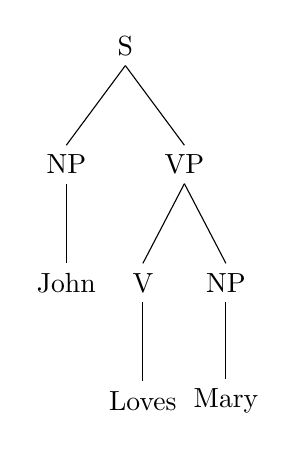
\begin{tikzpicture}
%[node distance = 0 pt, sibling distance=40pt, level distance=40pt,level 2/.style={sibling distance=9pt},level 3/.style={sibling distance=9pt}]
[level 2/.style={sibling distance = 30 pt}]

\node (S) {S}
child { node {NP}  
	child{ node {John}}
	}
child { node {VP} 
	child{ node {V} 
		child {node {Loves}}
		} 
	child{node {NP}
		child {node {Mary}}
		}
	}
;
\end{tikzpicture}

\end{figure}
  \end{itemize}
\end{frame}

\begin{frame}{Grammar}
A grammar describes:
\begin{itemize}
\item how trees can be built
\begin{itemize} 
\item CFG's - elementary rules
\item TSG's  - larger units: \emph{fragments}
\end{itemize}
\item how likely constructions are: \emph{probabilistic} grammars
\begin{itemize} 
\item PCFG's - independence 
\item PTSG's  - derivations
\end{itemize}

\end{itemize}
\end{frame}

\begin{frame}{Grammar: CFG rules}
\begin{quotation}
S\pijl{} NP VP\\
VP\pijl{} V NP\\
NP \pijl{} John\\
NP\pijl{} Mary\\
V\pijl{} loves
\end{quotation}

\end{frame}
\begin{frame}{Grammar: Tree fragments}

\begin{figure}
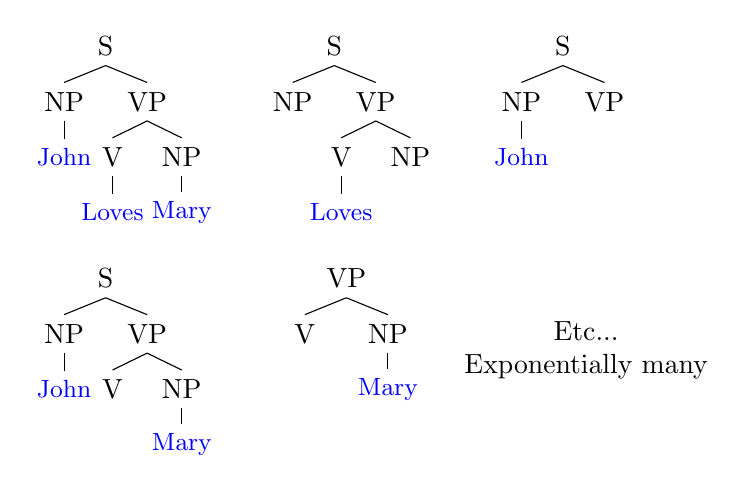
\begin{tikzpicture}
[node distance = 70 pt, sibling distance=30pt, level distance=20pt,level 2/.style={sibling distance=25pt},level 3/.style={sibling distance=15pt}]
%[level 2/.style={sibling distance = 30 pt}]

\node (f1) {S}
child { node {NP}  
	child{ node [color=blue]{\small John}}
	}
child { node {VP} 
	child{ node {V} 
		child {node [color=blue]{\small Loves}}
		} 
	child{node {NP}
		child {node [color=blue]{\small Mary}}
		}
	};
\node (f2)[right=of f1] {S}
child { node {NP} 
	}
child { node {VP} 
	child{ node {V} 
		child {node [color=blue]{\small Loves}}
		} 
	child{node {NP}
		}
	};
\node (f3)[right=of f2] {S}
child { node {NP}  
	child{ node [color=blue]{\small John}}
	}
child { node {VP} 
	};

\node (f4)[below=of f1] {S}
child { node {NP}  
	child{ node [color=blue]{\small John}}
	}
child { node {VP} 
	child{ node {V} 
		} 
	child{node {NP}
		child {node [color=blue]{\small Mary}}
		}
	};

\node (f5)[right=of f4] {VP} 
	child{ node {V} 
		} 
	child{node {NP}
		child {node [color=blue]{\small Mary}}
		};
\node(etc)[below right = 0cm and 1cm of f5, align=center]{\\Etc...\\ Exponentially many};
\end{tikzpicture}

\end{figure}


\end{frame}

\begin{frame}{Grammar: Tree fragments}

\begin{figure}
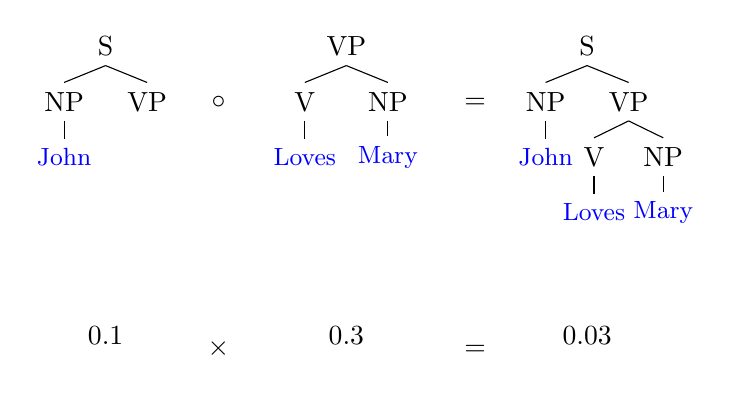
\begin{tikzpicture}
[node distance = 70 pt, sibling distance=30pt, level distance=20pt,level 2/.style={sibling distance=25pt},level 3/.style={sibling distance=15pt}]
%[level 2/.style={sibling distance = 30 pt}]

\node (f1) {S}
child { node {NP}  
  child{ node [color=blue]{\small John}}
  }
child { node {VP} };
\node(c)[below right = 0cm and 1cm of f1, align=center]{\\$\circ$};
\node (f2)[right=of f1] {VP} 
  child{ node {V} 
    child {node [color=blue]{\small Loves}}
    } 
  child{node {NP}
    child {node [color=blue]{\small Mary}}
    };
\node(is)[below right = 0cm and 1cm of f2, align=center]{\\$=$};
\node (f3)[right=of f2] {S}
child { node {NP}  
  child{ node [color=blue]{\small John}}
  }
child { node {VP} 
  child{ node {V} 
    child {node [color=blue]{\small Loves}}
    } 
  child{node {NP}
    child {node [color=blue]{\small Mary}}
    }
  };

\node(p1)[below=3cm of f1, align=center]{\\$0.1$};
\node(p2)[below=of c, align=center]{\\$\times$};
\node(p3)[below=3cm of f2, align=center]{\\$0.3$};
\node(p4)[below=of is, align=center]{\\$=$};
\node(p5)[below=3cm of f3, align=center]{\\$0.03$};

\end{tikzpicture}

\end{figure}


\end{frame}


\subsection{Bias and Consistency}

\begin{frame}{Consistency}

\begin{itemize}
\item Assumption
  \begin{itemize}
  \item Language is an infinite parse tree distribution
  \item Treebank is a finite sample
  \end{itemize}
\item \emph{Estimate} the true distribution
\item Expected estimation should improve when the treebank grows 
$\rightarrow$ expected \emph{loss} should decline
\item {\bf Consistency}: Expected loss becomes 0 when the sample size approaches $\infty$
\end{itemize}
\end{frame}


\begin{frame}{Bias}

\begin{itemize}
\item Assumption
  \begin{itemize}
  \item An estimator should approach \emph{any} distribution
  \item Even finite distributions!
  \end{itemize}
\item If there's a distribution that doesn't match its expected estimate, the estimator is {\bf biased}.
\item What about unseen data?
\item Bias is {\bf good}
\end{itemize}
\end{frame}

\section{\ddop{} and \dops{}: a comparison}

\subsection{Introduction to \ddop{} and \dops{}}
\begin{frame}{\ddop{}}
\begin{itemize}
\item Extraction: Maximal Overlap
\item Estimation: relative frequency 
\item Coverage: PCFG rules
\end{itemize}
\end{frame}

\begin{frame}{\dops{}}
\begin{itemize}
\item Held-out estimation - $HC$ and $EC$
\item Extraction: Shortest derivations
\item Estimation: relative frequency \emph{in shortest derivations}
\item Coverage: smoothing PCFG rules with probability $p_{unkn}$
\end{itemize}
\end{frame}

\subsection{Comparison}
\begin{frame}{Comparison}
\begin{itemize}
\item Shortest derivations or Maximal overlap
\item Held-out estimation or one vs. the rest
\end{itemize}
\end{frame}

\subsection{Experiments}
\begin{frame}{Three grammars}
\begin{itemize}
\item Shortest derivations (split)
\item Maximal overlap (full)
\item Maximal overlap (split)
\end{itemize}
\end{frame}


\section{Results}
\begin{frame}
\begin{figure}[h!]
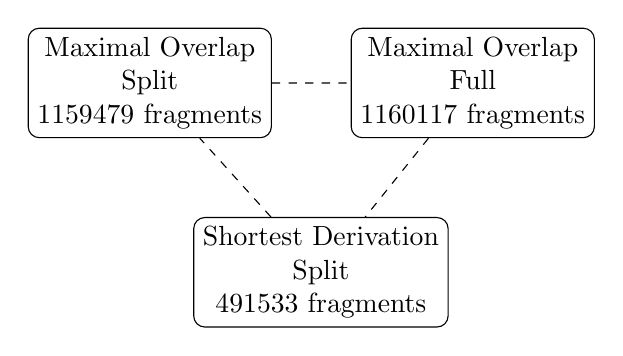
\begin{tikzpicture}[node distance = 1cm]
\node (MOS) [rectangle,rounded corners,draw, align=center]{Maximal Overlap\\ Split\\1159479 fragments};
\node (MOF) [right = of MOS, rectangle,rounded corners,draw, align=center]{Maximal Overlap\\ Full\\1160117 fragments};
\node (SDS) [below right= 1 cm and -1 cm of MOS, rectangle,rounded corners,draw, align=center]{Shortest Derivation\\ Split\\491533 fragments};
\draw[dashed](MOS)--(MOF)--(SDS)--(MOS);
\end{tikzpicture}
\caption{The grammars and their size}
\label{f:grammars}
\end{figure}
\end{frame}


\subsection{Analyzing grammars}

\begin{frame}{Maximal overlap $\leftrightarrow$ shortest derivation}
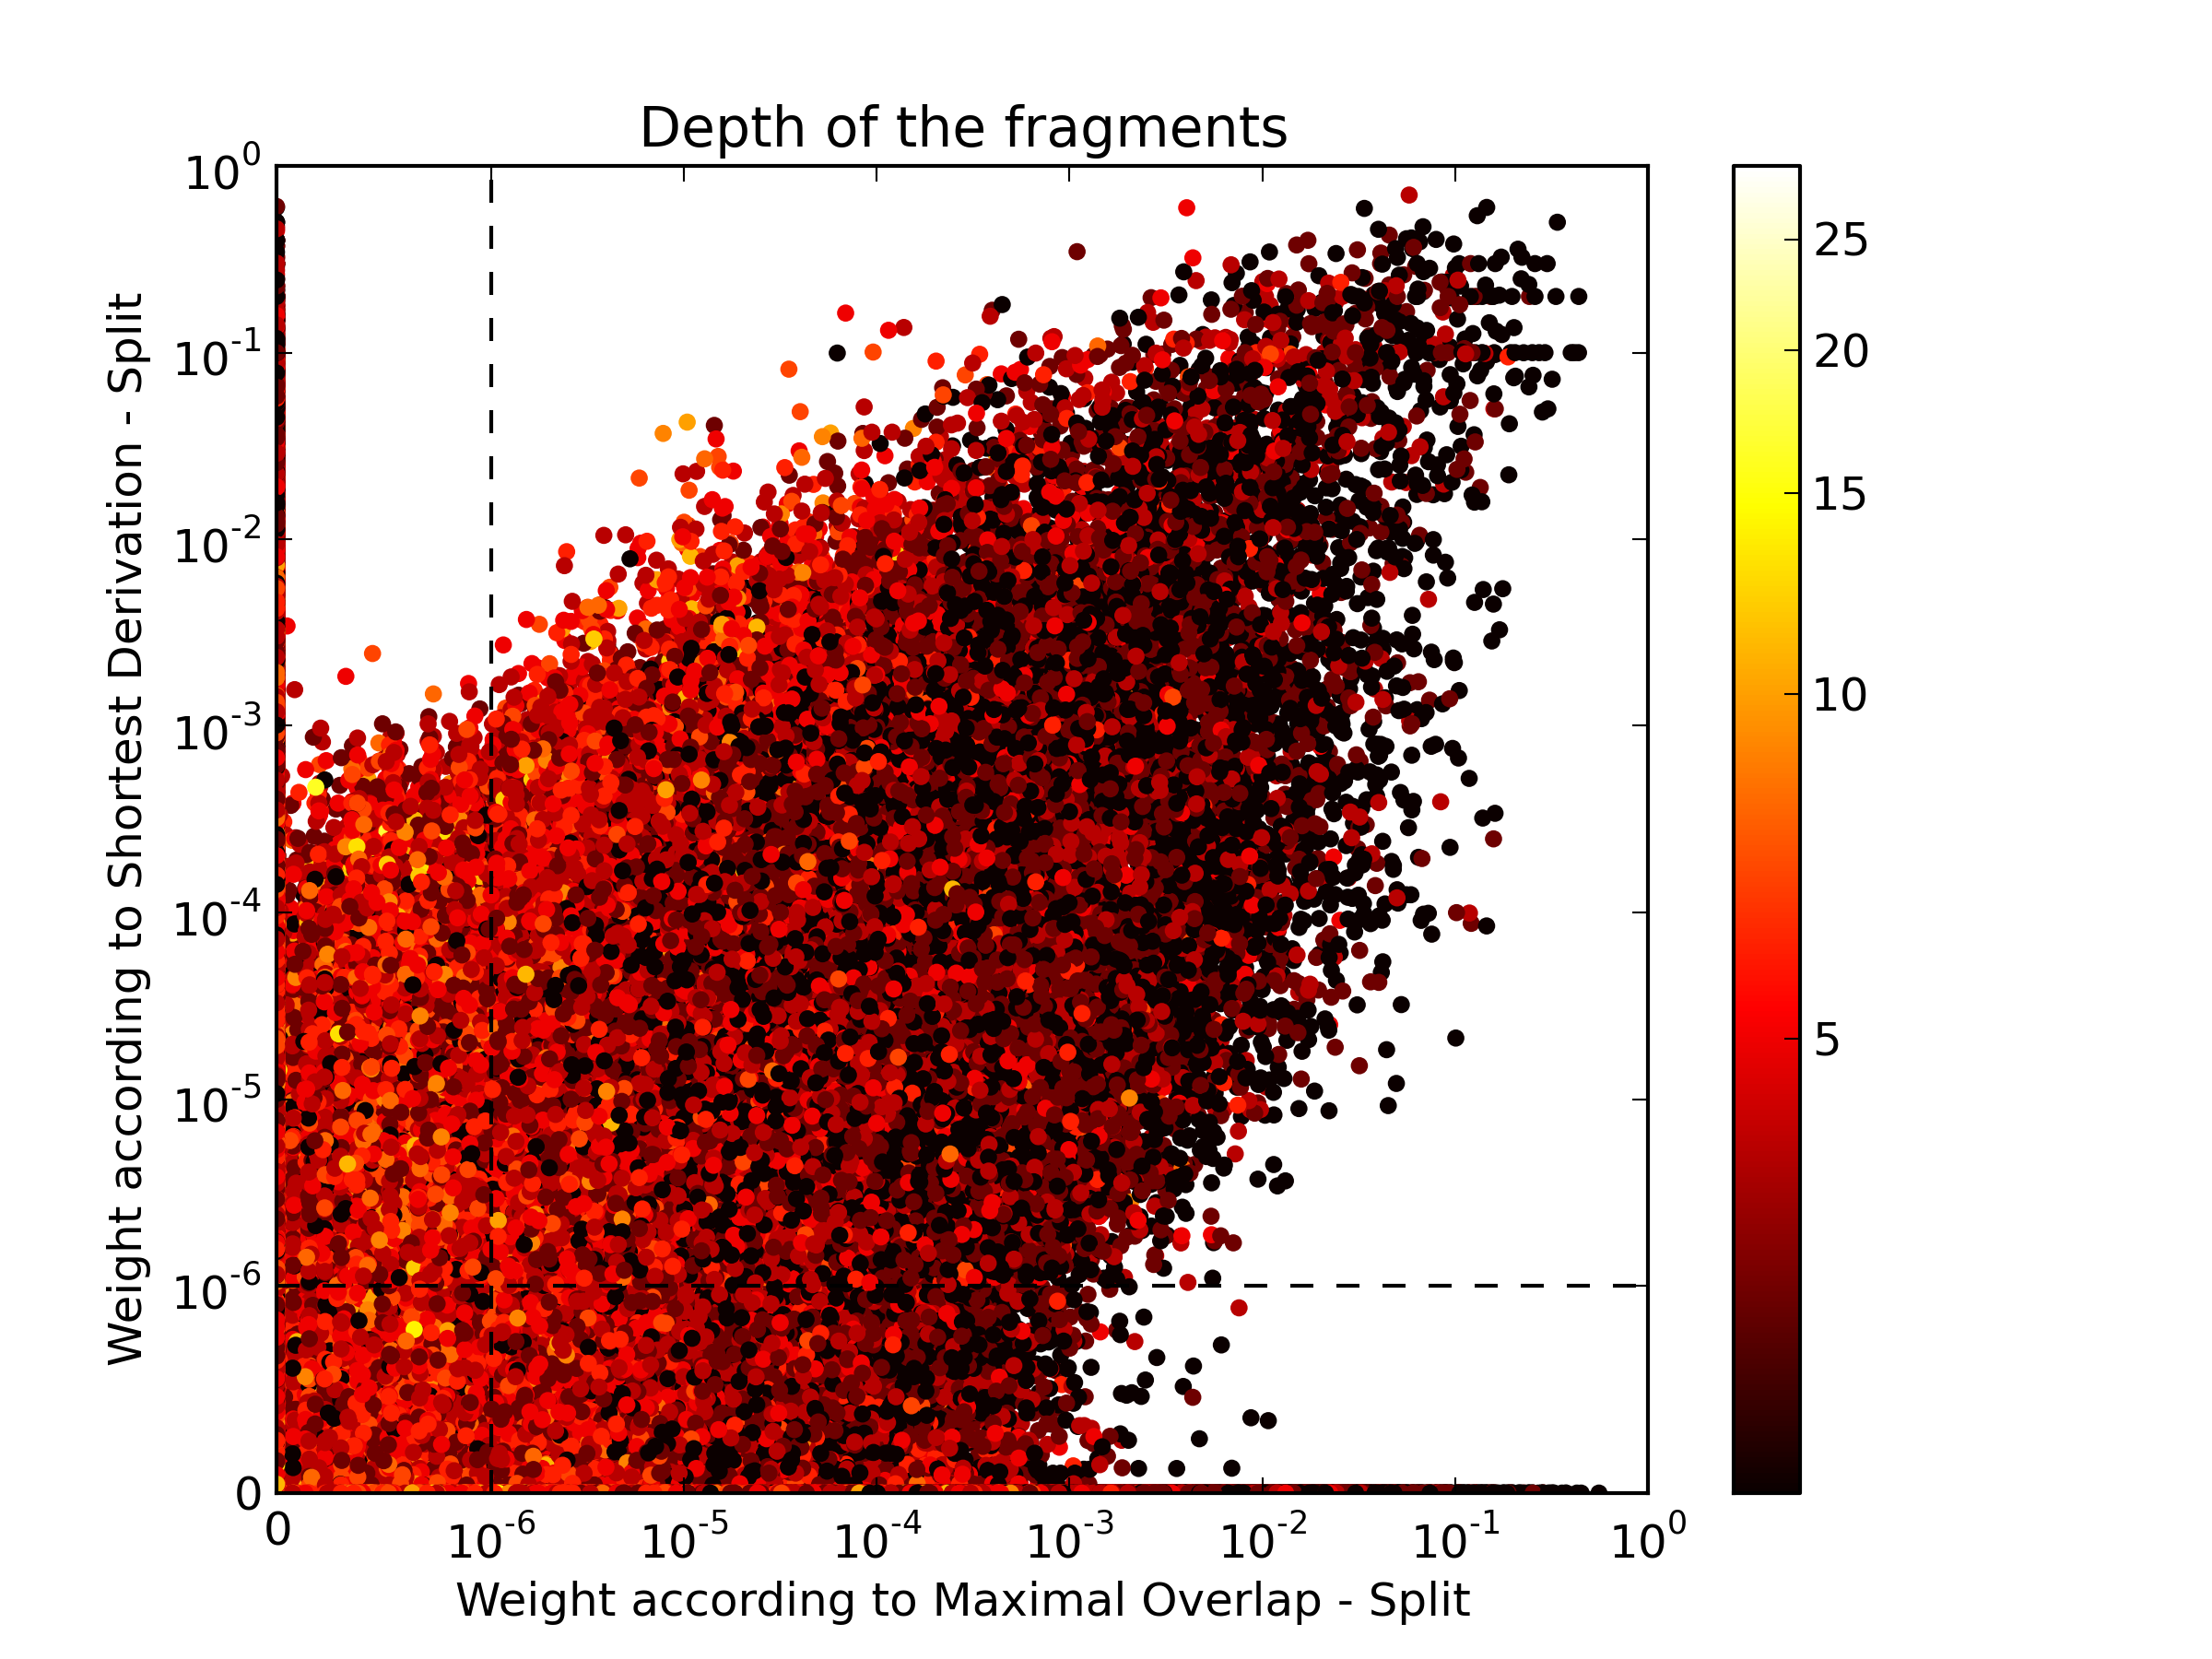
\includegraphics[width=\linewidth,trim=0.5cm 0cm 2.5cm 0.5cm, clip=true]{../data/plots/0.png}
\end{frame}

\begin{frame}{Split $\leftrightarrow$ one vs. the rest}
\end{frame}

\subsection{Parsing Performance}
\begin{frame}{F1 scores}
\end{frame}


\section*{Summary}

\begin{frame}{Summary}

  % Keep the summary *very short*.
  \begin{itemize}
  \item
    So \alert{shortest derivations} are not as useful as they seem
  \item
    And a \alert{split} moves weight to large fragments
  \item
    \alert{Performance} is not related to \alert{consistency}
  \end{itemize}
  
  % The following outlook is optional.
  \vskip0pt plus.5fill
  \begin{itemize}
  \item
    Outlook
    \begin{itemize}
    \item
      Why not?
    \item
      Is it just grammar size?
    \end{itemize}
  \end{itemize}
\end{frame}

\bibliographystyle{acl2014}
\bibliography{bibliography}


%
%
%% All of the following is optional and typically not needed. 
%\appendix
%\section<presentation>*{\appendixname}
%\subsection<presentation>*{For Further Reading}
%
%\begin{frame}[allowframebreaks]
%  \frametitle<presentation>{For Further Reading}
%    
%  \begin{thebibliography}{10}
%    
%  \beamertemplatebookbibitems
%  % Start with overview books.

  % \bibitem{Author1990}
  %   A.~Author.
  %   \newblock {\em Handbook of Everything}.
  %   \newblock Some Press, 1990.
 
    
  % \beamertemplatearticlebibitems
  % % Followed by interesting articles. Keep the list short. 

  % \bibitem{Someone2000}
  %   S.~Someone.
  %   \newblock On this and that.
  %   \newblock {\em Journal of This and That}, 2(1):50--100,
  %   2000.
  % \end{thebibliography}
% \end{frame}

\end{document}


